\section{Implementierung}
\subsection{Screenshots}
\begin{frame}
\begin{figure}
   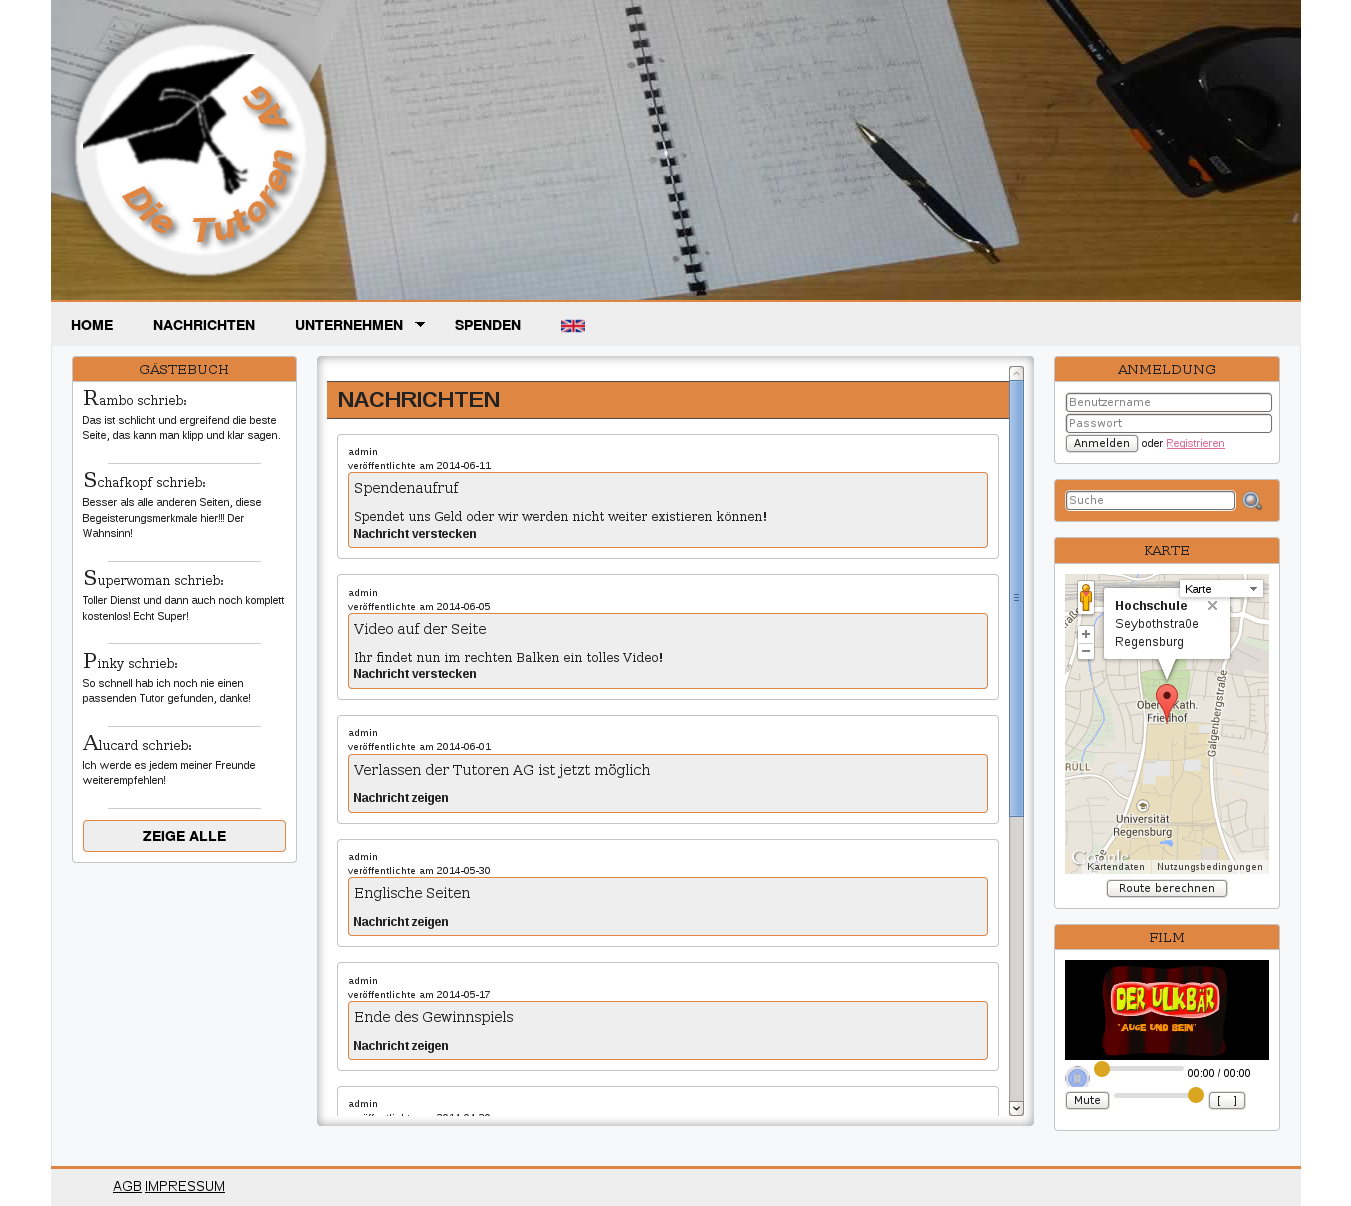
\includegraphics[width= 0.8\paperwidth]{Nachrichten.png}
\end{figure}
\end{frame}

\begin{frame}
\begin{figure}
   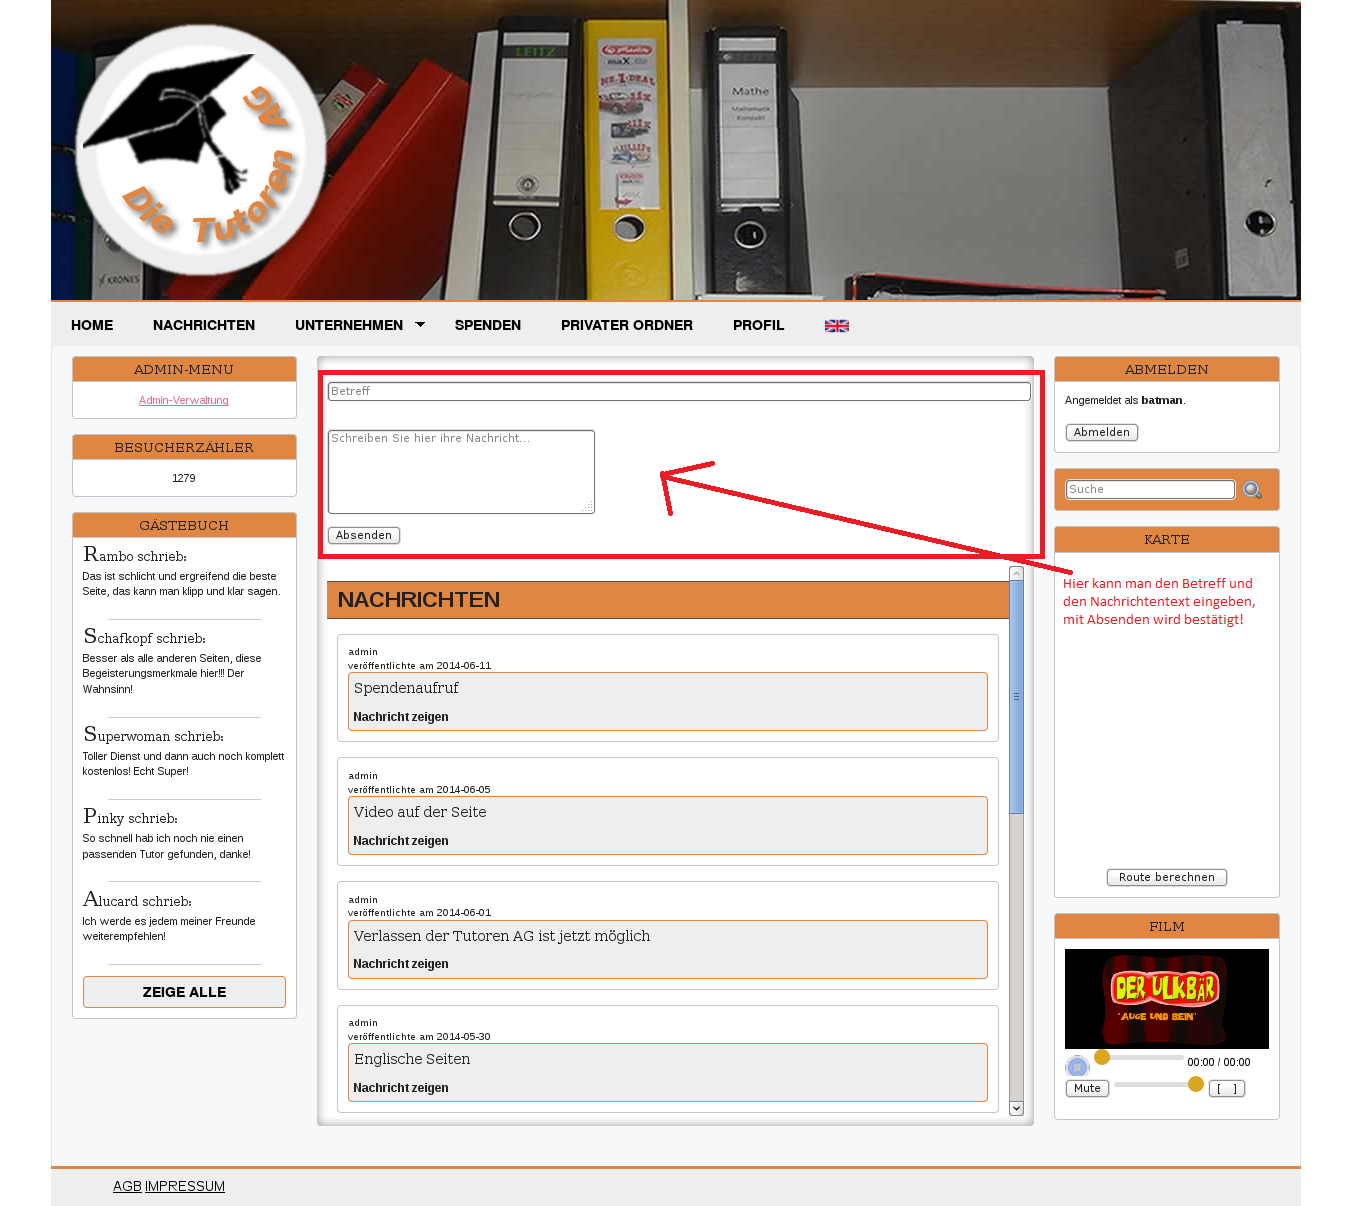
\includegraphics[width= 0.8\paperwidth]{Nachrichten_admin.png}
\end{figure}
\end{frame}
\subsection{Code}

\defverbatim[colored]
  \makeset{
    \phpcode
	\lstset{language=html}
      \begin{lstlisting}
<div style="height:200px;">
        <form name="News" id="newsform">
            <script src="/js/newsvalidation.js" type="text/javascript"></script>
            <input type="hidden" name="sprache" value="<?php echo $_SESSION['sprache']; ?>">
            <input type="hidden" name="user" value="<?php echo $_SESSION['user']; ?>">
            <div><label for ="betreff"></label><input type="text" size="44" maxlength = "60" placeholder = "Betreff" name="subject" id="betreff" required></div>
            <div><label for ="nachrichtentext"></label>
                <p><textarea name="nachricht" cols="33" rows="5" maxlength="300" id="nachrichtentext" placeholder ="Schreiben Sie hier ihre Nachricht..." required></textarea>
                </p>
            </div>
            <div class="line submit"><input type="submit" value="Absenden"></div>
        </form>
    </div>
    <script>
        $(document).ready(function() {
            $("#scrollablecontentboxnews_de").height(550);
        });
    </script>

    

      \end{lstlisting}
}

\begin{frame}
  \frametitle{Formular}
  \makeset
\end{frame}



\defverbatim[colored]
  \makeset{
    \phpcode
      \begin{lstlisting}
<?php 
	[...]
	try {
		$dbConnection = ConnectToDB();
	} catch (Exception $e) {
		die("keine Verbindung moeglich: " . $e->getMessage());
	}
	[...]
	$dbConnection->setAttribute(PDO::ATTR_CASE, PDO::CASE_NATURAL);
		
	$query = $dbConnection->prepare("insert into news (benutzername, zeit, nachricht, betreff) VALUES ( :user, CURRENT_DATE, :msg, :subject)");
		
	$query->bindParam(":msg", $msg);
	$query->bindParam(":user", $_POST['user']);
	$query->bindParam(":subject", $subject);
		
	$query->execute();
	$dbConnection = null;
?>
      \end{lstlisting}
}

\begin{frame}
  \frametitle{WriteNews.php}
	\makeset
\end{frame}


\defverbatim[colored]
  \makeset{
    \phpcode
      \begin{lstlisting}
<?php
	[...]
	
    $query = $dbConnection->prepare("SELECT * FROM news where 1 order by id desc");
    $query->execute();
    $results = $query->fetchAll(PDO::FETCH_ASSOC);
     	
    echo json_encode($results);
     	
    $dbConnection = null;
?>
     
      \end{lstlisting}
}

\begin{frame}
  \frametitle{ReadNews.php}
  \makeset
\end{frame}




\subsection{Demonstration}
\begin{frame} %%Eine Folie
%   \frametitle{Analyse} %%Folientitel

% Fettgedruckt
  \textbf{Es folgt eine Demonstration ...}
\end{frame}
